\chapter{Related Work}

% TODO: SAVE??? KILL?? YOU DECIDE!

\section{Spaced Repitition Apps}
\subsection{Duolingo}

\begin{figure}
	%\centering
	\centerline{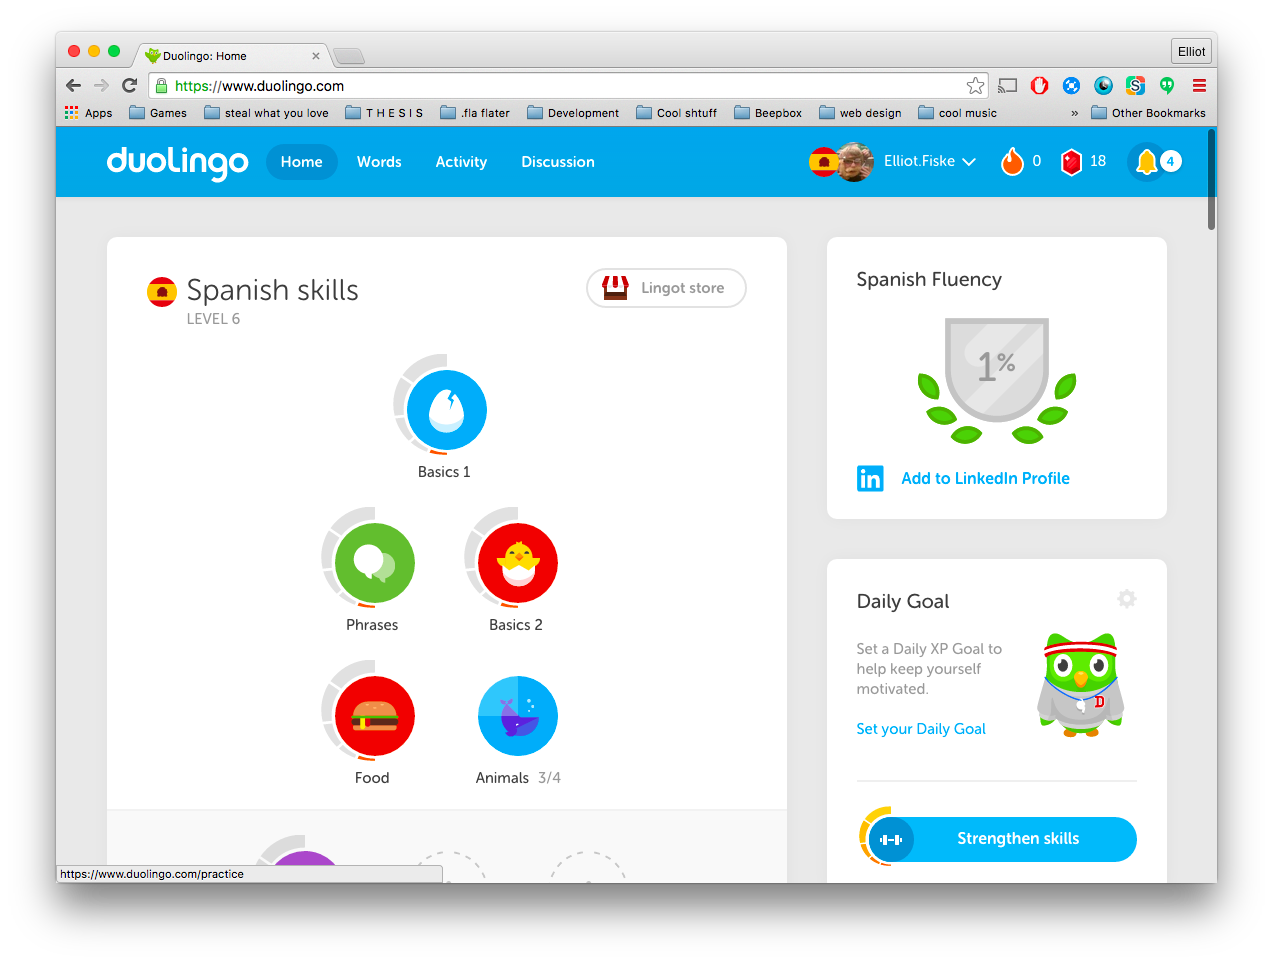
\includegraphics[width=1.2\linewidth]{duolingo}}
	\caption[Duolingo]{The Duolingo interface. Notice the gamification elements and the encouragement to reach a "daily goal."}
	\label{fig:duolingo}
\end{figure}

\par Several recent apps and products make use of spaced repetition to allow user to easily gain long-term recall of languages, class content, or any other information that needs to be learned. One such app is Duolingo (See \textbf{\hyperref[fig:duolingo]{Figure \ref*{fig:duolingo}}}); in Duolingo, users learn a language by repeating small exercises every day. 

\par The app encourages users to spend a small amount of time each day studying useful words and phrases, rather than cramming in a lot of knowledge at once. It encourages this behavior through the use of gamification. Each user earns "experience" in a language, eventually leveling up. Users connect their Facebook accounts and can see their friends' levels and accomplishments, adding a social element to the app. % TODO: Expand on this yo.

\subsection{Memrise}

\begin{figure}
	\centering
	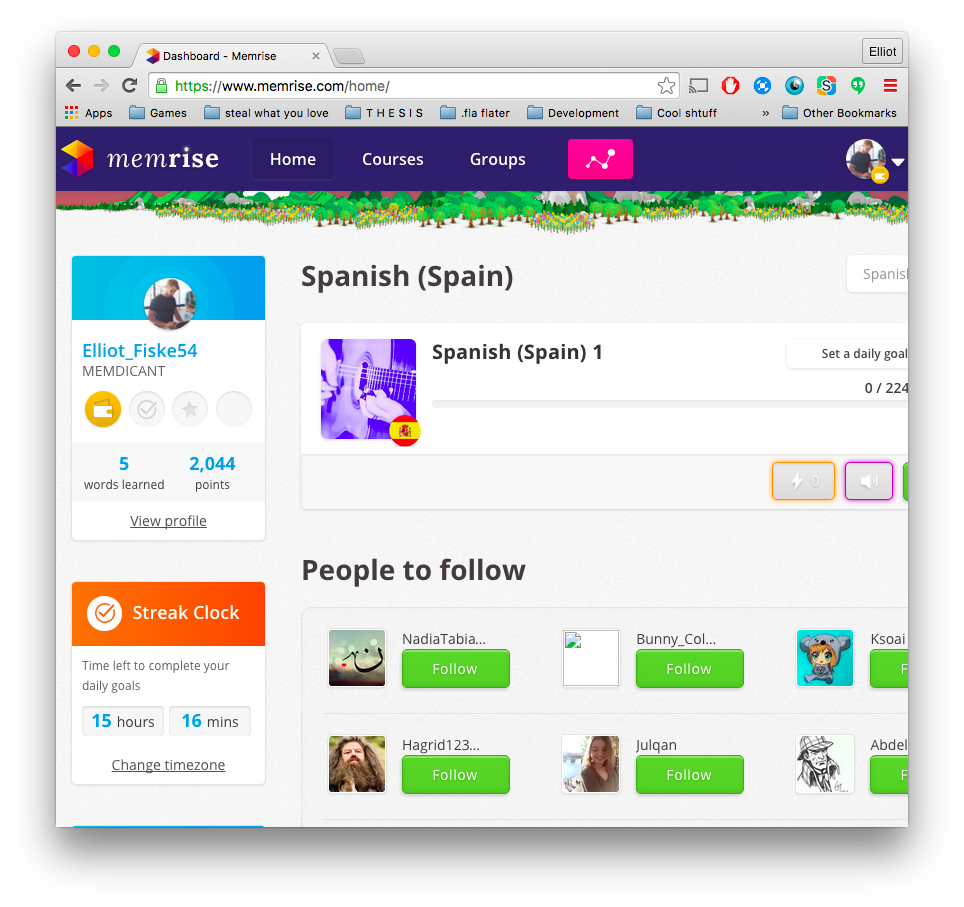
\includegraphics[width=0.7\linewidth]{memrise}
	\caption[Memrise]{Screenshot of the Memrise interface. Note the gamification elements, the social aspect, and the "Streak" clock encouraging consistent use of the app.}
	\label{fig:memrise}
\end{figure}

\par Memrise (See \textbf{\hyperref[fig:memrise]{Figure \ref*{fig:memrise}}}) is a web app that has very similar function to \textit{Commit.} Memrise takes a series of flashcard-based questions and answers and automatically creates a "study plan" where the application breaks up flash cards and uses spaced repitition to encode the information in the user's long-term memory. Memrise also uses gamification and social elements, as users earn points for every correct answer and can see their friends' scores.

\par Interesting to note is that users can input any data they choose into Memrise to receive a custom study-guide. This would allow students to easily learn flashcards if they took the time to input them into the app.

\par Both of these applications heavily emphasize language learning, since the process of learning a language can easily be broken down into a series of small words and phrases, and re-emphasized using the process of spaced repetition. However, Commit is scoped specifically to one class, allowing students to easily learn and retain class content without the commitment of adding their own flashcards.

% end stuff


\section{Habit Formation}

\subsection{Pocket Points}
\par Pocket Points is an app that attempts to create positive habits for its users through gamification \cite{pocketpoints}. When installed, the app rewards you for keeping your phone locked while in class. It uses GPS to ensure you're on campus, then awards 1 point for every 20 minutes your phone is locked. These points can then be spent to earn discounts and coupons at local businesses.

\par Pocket Points has the benefit of providing a 
TODO: FINISH THIS SECTION ON POCKET POINTS


\begin{figure}
	\centering
	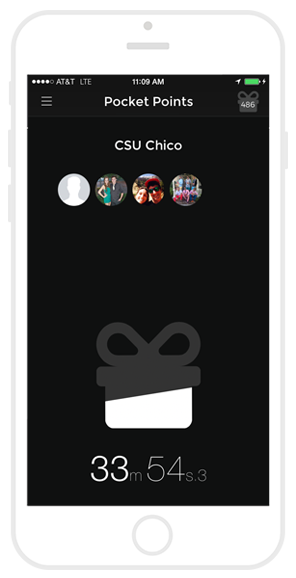
\includegraphics[width=0.7\linewidth]{figures/pocket-points}
	\caption[Memrise]{Screenshot of the Pocket Points interface. }
	\label{fig:pocket-points}
\end{figure}


\subsection{Habit Formation and User Interface}
Previous work has been done to tie habit formation with online user interfaces \cite{johnson2013designing}. In this book, Dr. Jeff Johnson describes how psychology ties into user interface design. He cites that familiar user interfaces lead to less mental stress, encouraging users to come back to your application repeatedly since it seems familiar and less stressful to them. We desire users to consistently use our application every day, so we must keep this in mind. 

\subsection{Memrise}
As mentioned before, Memrise is an excellent example of habit formation. In one paper, researchers gauged the ability of students to memorise simple Latin phrases in a classroom setting. They found that Memrise is an effective tool 

\section{Gamification}
Gamification in the classroom has several other examples that can be compared to our application.

\subsection{Classcraft}
Classcraft is an intriguing example of gamification in education (See \textbf{\hyperref[fig:classcraft]{Figure \ref*{fig:classcraft}}}). In Classcraft, students choose a "role" and go on the equivalent of a World of Warcraft raid with their fellow classmates. Classcraft is interesting in that it promotes co-operation and a variety of skills, so that students can assist each other where they might not have a certain skill. 

Classcraft takes the typical elements of an RPG and converts them into an experience that supplements a typical classroom experience.

\begin{figure}[h]
	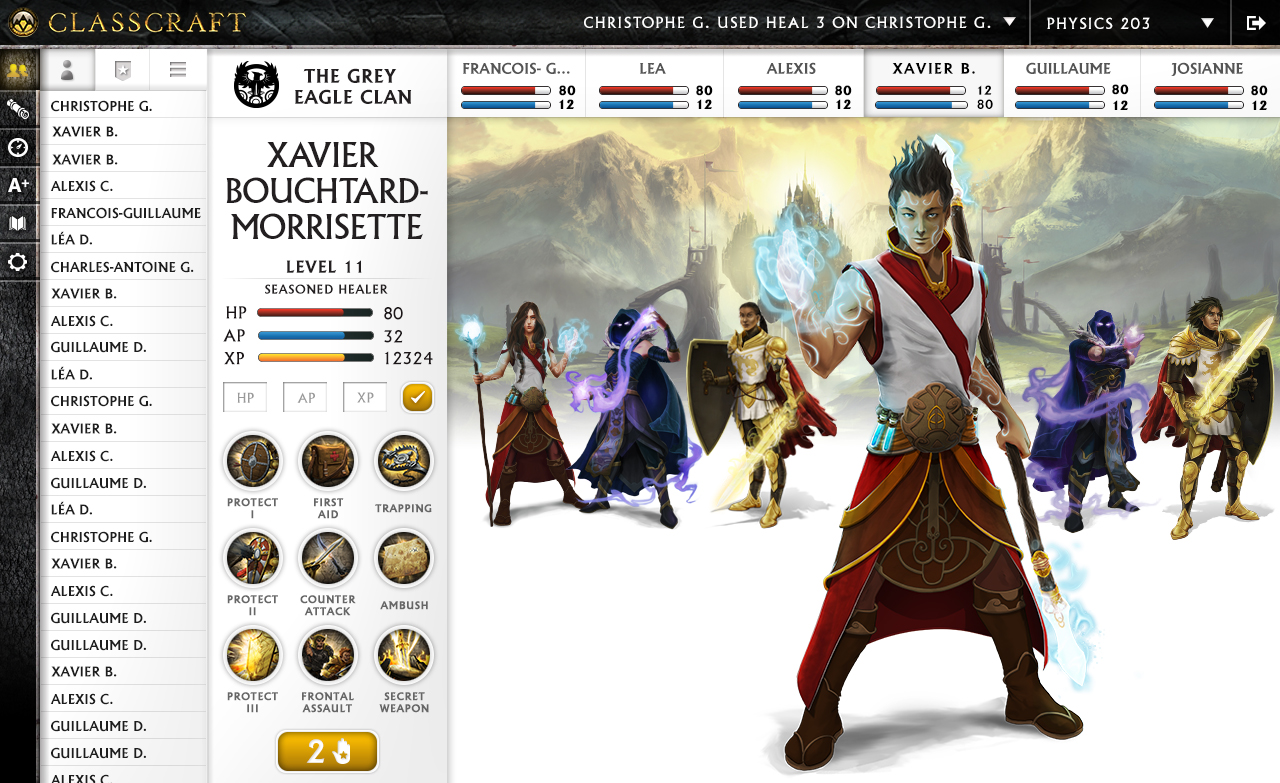
\includegraphics[width=1.0\linewidth]{figures/classcraft}
	\caption{Classcraft user interface. Note the student's health and mana pool, as well as the list of other students in the classroom.}
	\label{fig:classcraft}
	\cite{hardy_heyes_1999}
\end{figure}

Interesting to note is the emphasis Classcraft puts on integration with existing technologies such as Google Classroom. In order for this application to be widely adopted, it is definitely necessary to have the experience of the teacher go extremely smoothly. Thus, if an application ties directly in with existing technology that the teacher is already familiar with, it will be much more readily adopted by the educational community. It's important to value the teacher's time with this application, so it is necessary to make the UI recognizable, familiar and easy to work with, as well as integrating it with existing tools and perhaps even modeling the user interface after tools that many teachers will already be familiar with.

\subsection{Classcraft Study}
A study was done on the effectiveness of Classcraft as well as "ludicization" in the classroom in general \cite{sanchez2016classcraft}. Their study ran primarily in France, as this is the home country of the Classcraft company and application.

%TODO
TODO: update classcraft stuff

\subsection{Gamification in Other Educational Areas}
So far, we have considered gamification in the classroom mostly in the context of STEM or language fields. While gamification does lend itself towards these subjects, as math problems and science problems can be easily generated by an algorithm, there have also been steps to gamify aspects of classes around liberal arts and the humanities \cite{wagner2017digital}. 

This study by Dr. Wagner approaches a music class the same way Classcraft approaches subjects not focused on the humanity. It highlights the idea of a "flow" where a student is fully immersed in the educational process and is fully engaged with the learning process, and notes that it is far easier to attain this "flow" state when the student is learning in the context of a video game.